\documentclass{beamer}
\usetheme{Madrid}

\usepackage{amsmath, amssymb, amsthm}
\usepackage{graphicx}
\usepackage{listings}
\usepackage{gensymb}
\usepackage{minted}
\usemintedstyle{friendly}
\definecolor{bg}{rgb}{0.95,0.95,0.95}
\usepackage[utf8]{inputenc}
\usepackage{hyperref}
\usepackage{gvv}\begin{document}
\title{7-7.3-3}
\author{EE24BTECH11058 - SHINY DIAVAJNA}
\date{6 November,2024}
\frame{\titlepage}

\begin{frame}
\frametitle{Question}
 The equation of a circle with origin as centre and passing through the vertices of an equilateral triangle whose median is of length 3a is \\
\end{frame}
\begin{frame}{allowframebreaks}
\frametitle{Table}
\begin{table}[h!!]
    \centering
    \begin{tabular}[12pt]{ |c|c|c|}
    \hline
	\textbf{Symbol} & \textbf{Description} & \textbf{Value}\\
    \hline
	$\vec{O}$ & Centre of the circle &\myvec{0 \\ 0} \\
    \hline 
	$3a$ & median of the triangle & -  \\
    \hline
	$r$  & radius of the circle & - \\
    \hline
	$u$  & $-O$ & $\myvec{0 \\ 0}$\\
    \hline
        $f$ & ${\norm{u}}^2 - {r}^2 $ & - \\
    \hline
    \end{tabular}
    \caption{Variables Used}
    \label{tab 7.7.3.3}
\end{table}
\end{frame}

\begin{frame}
\frametitle{Theory}
  \begin{itemize}
      \item General equation of a conic is $g\brak{x} = x^\top V x + 2 u^\top x+f =0$
      
      \item For a circle $V = \myvec{1 & 0 \\ 0 & 1}$
      
      \item Therefore, general equation of a circle is \\
           \begin{align}
               {\norm{x}}^2 + 2 u^\top x+f =0 \\
               u = -O  ,  f = {\norm{u}}^2 - {r}^2 
           \end{align}\\
           
   \end{itemize}
\end{frame}

\begin{frame}
\frametitle{Theory}

     \begin{itemize}

     \item The circumcircle of a triangle is the unique circle that passes through all three vertices of the triangle. The center of this circle is called the circumcenter.
     
    \item   In an equilateral triangle, the centroid, circumcenter, and incenter are all the same point.
    
    \item  The centroid divides each median in a 2:1 ratio (measured from the vertex to the midpoint of the opposite side).
    
    \item  Therefore, the centre of the circle divides the median in the ratio 2:1. Hence,radius of the cirle is 2a.
    \end{itemize}
    
\end{frame}

\begin{frame}
\frametitle{Solution}
\begin{align}
   \text{The general equation of a circle }\\
{\norm{x}} ^ 2 + {u}^\top x + f =0\\
u = \myvec {0\\ 0}\\
r = 2a\\
f = {\norm{u}}^2 - {r}^2 \\
f = -4 {a} ^2\\
{\norm{x}} ^ 2 - 4a ^2 =0\\
x^2 + y^2 = 4a^2
\end{align}
\end{frame}
 
 
\begin{frame}
\frametitle{Figure}
\begin{figure}
    \centering
    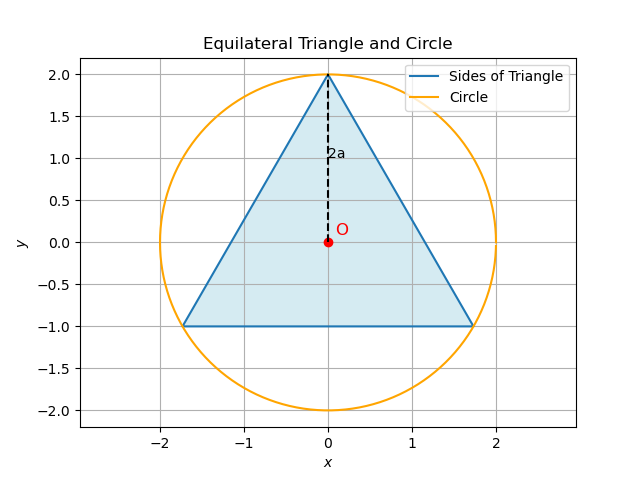
\includegraphics[width=0.7\linewidth]{Figure_1.png}
     
\end{figure}
\end{frame}
\begin{frame}[fragile]
\frametitle{C-Code}
\begin{minted}[bgcolor=bg, linenos, fontsize=\small, breaklines]{c}
#include <stdio.h>
#include <stdlib.h>
#include <math.h>
#include "libs/matfun.h"
#include "libs/geofun.h"

void point_gen(FILE *fptr, double **A, double **B, int no_rows, int no_cols, int num_points) {
    for (int i = 0; i < num_points; i++) {
        double t = (double)i / (num_points - 1);
        double **output = Matadd(A, Matscale(Matsub(B, A, no_rows, no_cols), no_rows, no_cols, t), no_rows, no_cols);
        fprintf(fptr, "%lf,%lf\n", output[0][0], output[1][0]);
        freeMat(output, no_rows);
    }
}
\end{minted}
\end{frame}
\begin{frame}[fragile]
\frametitle{C-Code}
\begin{minted}[bgcolor=bg, linenos, fontsize=\small, breaklines]{c}
    void equi_triangle_gen(double median, FILE *fptr) {
    double side = (2 * median) / sqrt(3);
    double xA = 0, yA = 2*median/3;
    double xB = -side / 2, yB = -median/3;
    double xC = side / 2, yC =  -median/3;
    
    int m = 2, n = 1;
    
    double **A = createMat(m, n);
    double **B = createMat(m, n);
    double **C = createMat(m, n);
    
    A[0][0] = xA;  A[1][0] = yA;
    B[0][0] = xB;  B[1][0] = yB;
    C[0][0] = xC;  C[1][0] = yC;

\end{minted}
\end{frame}

\begin{frame}[fragile]
\frametitle{C-Code}
\begin{minted}[bgcolor=bg, linenos, fontsize=\small, breaklines]{c}
    point_gen(fptr, A, B, m, n, 10);
    point_gen(fptr, B, C, m, n, 10);
    point_gen(fptr, C, A, m, n, 10);

    freeMat(A, m);
    freeMat(B, m);
    freeMat(C, m);
}

void circle_point_gen(FILE *fptr, double radius, double *center, int num_points) {
    double **output;
    for (int i = 0; i < num_points; i++) {
        double angle = (2 * M_PI * i) / num_points;
        output = createMat(2, 1);
        output[0][0] = center[0] + radius * cos(angle);
        output[1][0] = center[1] + radius * sin(angle);

\end{minted}
\end{frame}

\begin{frame}[fragile]
\frametitle{C-Code}
\begin{minted}[bgcolor=bg, linenos, fontsize=\small, breaklines]{c}
   fprintf(fptr, "%lf,%lf\n", output[0][0], output[1][0]);
        freeMat(output, 2);
    }
}

int main() {
    double a = 1.0; //for graphing
    double median = 3*a;
    double radius = 2*a; 
    double center[2] = {0.0, 0.0};

    FILE *fptr = fopen("points.dat", "w");
    if (fptr == NULL) {
        printf("Error opening file!\n");
        return 1;
    }

    
\end{minted}
\end{frame}

\begin{frame}[fragile]
\frametitle{C-Code}
\begin{minted}[bgcolor=bg, linenos, fontsize=\small, breaklines]{c}
    equi_triangle_gen(median, fptr);
    circle_point_gen(fptr, radius, center, 300);

    fclose(fptr);
    return 0;
}
\end{minted}
\end{frame}



\begin{frame}
\frametitle{C code output}
 0.000000,2.000000 \\
-0.192450,1.666667 \\
-0.384900,1.333333\\
-0.577350,1.000000\\
-0.769800,0.666667\\
-0.962250,0.333333\\
-1.154701,0.000000\\
-1.347151,-0.333333\\
-1.539601,-0.666667\\
-1.732051,-1.000000\\
-1.732051,-1.000000\\
-1.347151,-1.000000\\
-0.962250,-1.000000\\
-0.577350,-1.000000\\
-0.192450,-1.000000\\

\end{frame}

\begin{frame}
\frametitle{C code output}
0.192450,-1.000000\\
0.577350,-1.000000\\
0.962250,-1.000000\\
1.347151,-1.000000\\
1.732051,-1.000000\\
1.732051,-1.000000\\
1.539601,-0.666667\\
1.347151,-0.333333\\
1.154701,0.000000\\
0.962250,0.333333\\
0.769800,0.666667\\
0.577350,1.000000\\
0.384900,1.333333\\
0.192450,1.666667\\
0.000000,2.000000\\
 
\end{frame}

\begin{frame}
\frametitle{C code output}
2.000000,0.000000\\
1.999561,0.041885\\
1.998246,0.083751\\
1.996053,0.125581\\
1.992986,0.167356\\
1.989044,0.209057\\
1.984229,0.250666\\
1.978545,0.292166\\
1.971992,0.333537\\
1.964575,0.374763\\
1.956295,0.415823\\
1.947158,0.456702\\
1.937166,0.497380\\
1.926325,0.537840\\
1.914639,0.578064\\
1.902113,0.618034\\

\end{frame}

\begin{frame}
\frametitle{C code output}
1.888753,0.657733\\
1.874564,0.697144\\
1.859553,0.736249\\
1.843726,0.775031\\
1.827091,0.813473\\
1.809654,0.851559\\
1.791424,0.889270\\
1.772407,0.926592\\
1.752613,0.963507\\
1.732051,1.000000\\
1.710729,1.036054\\
1.688656,1.071654\\
1.665842,1.106783\\
1.642298,1.141427\\
1.618034,1.175571\\
1.593060,1.209198\\

\end{frame}

\begin{frame}[fragile]
  \frametitle{Python Code }

\begin{minted}[bgcolor=bg, linenos, fontsize=\small, breaklines]{python}
import numpy as np
import matplotlib.pyplot as plt

# Load data
points = np.loadtxt("points.dat", delimiter=',')
x_triangle = points[:30, 0]
y_triangle = points[:30, 1]
x_circle = points[30:, 0]
y_circle = points[30:, 1]

# Create the plot
plt.figure()
plt.plot(x_triangle, y_triangle, label='Sides of Triangle')
plt.fill(x_triangle, y_triangle, 'lightblue', alpha=0.5)
plt.plot(x_circle, y_circle, label='Circle', color='orange')



\end{minted}
\end{frame}
\begin{frame}[fragile]
  \frametitle{Python Code }

\begin{minted}[bgcolor=bg, linenos, fontsize=\small, breaklines]{python}
# Define circle center
circle_center = (0, 0)

# Indicate the center with a point and annotate it
plt.plot(circle_center[0], circle_center[1], 'ro')  # Red point for the center
plt.annotate('O', xy=circle_center, xytext=(5, 5), textcoords='offset points', fontsize=12, color='red')

# Identify the topmost vertex of the triangle (assuming it's the first vertex in your data)
top_vertex = (x_triangle[0], y_triangle[0])


                         
\end{minted}
\end{frame}

\begin{frame}[fragile]
  \frametitle{Python Code }
\begin{minted}[bgcolor=bg, linenos, fontsize=\small, breaklines]{python}

# Draw a line from the center to the top vertex
plt.plot([circle_center[0], top_vertex[0]], [circle_center[1], top_vertex[1]], 'k--')  # Dashed line
plt.annotate('2a', xy=((circle_center[0] + top_vertex[0]) / 2, (circle_center[1] + top_vertex[1]) / 2), 
                         fontsize=10, color='black')
                         
# Plot settings
plt.xlabel("$x$")
plt.ylabel("$y$")
plt.title("Equilateral Triangle and Circle")
plt.grid(True)
plt.legend(loc="upper right")
plt.axis('equal')
plt.show()

\end{minted}
\end{frame}


\end{document}
 
